\documentclass[11pt]{article}
\usepackage{bm}
\usepackage{ctex}
\usepackage{array}
\usepackage{float}
\usepackage{amssymb}
\usepackage{amsmath}
\usepackage{graphicx}
\usepackage{tabularx}
\usepackage{hyperref}
\usepackage{fancyhdr}
\usepackage{enumitem}
\usepackage{enumerate}
\pagestyle{fancy}
\hypersetup{hypertex = true,
			colorlinks = true,
			linkcolor = blue ,
			anchorcolor = blue,
			citecolor = blue}
\fancyhf{}
\chead{Compiler}
\fancyhead[r]{\bfseries\thepage}
\fancyhead[l]{\bfseries\rightmark}
\setlength{\listparindent}{0em} %段落缩进量
\begin{titlepage}
	\title{编译原理作业9}
	\author{
			\textbf{作者:} {吴润泽}
			\and {\textbf{学号:} 181860109}
		}
\end{titlepage}
\begin{document}
\maketitle
\section*{6.6.1 (2)}
\begin{table}[H]
	\begin{tabular}{|c|c|}
		\hline
		生成式&语义规则\\
		\hline
		$S\to \textbf{for}(S_1;B;S_2)S_3$&
		$\begin{aligned}
		&S_1.next=newlabel()\\
		&B.true=newlabel()\\
		&B.false=S.next()\\
		&S_2.next=S_1.next()\\
		&S_3.next=newlabel()\\
		&\begin{aligned}
		S.code=
		&S_1.code||label(S_1.next)\\
		&||B.code||label(B.true)\\
		&||S_3.code||label(S_3.next)\\
		&||S_2.code||gen('goto',S_1.next)
		\end{aligned}
		\end{aligned}
		$\\
		\hline
	\end{tabular}
\end{table}
\section*{6.7.1 (2)}
\subsection*{注释语法分析树}
\begin{figure}[H]
	\centering
	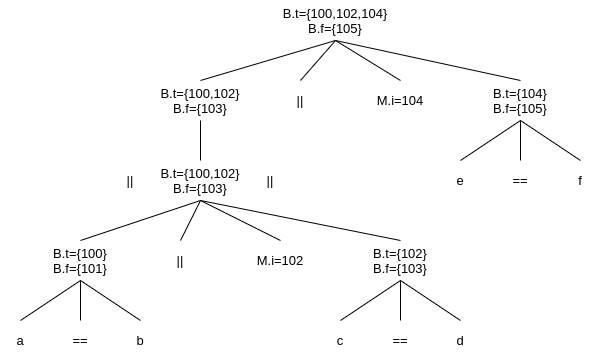
\includegraphics[width=\linewidth]{6.7.1-tree.png}
	%\caption{注释语法分析树}
\end{figure}
\subsection*{指令序列}
\begin{itemize}
	\item[100:] $\textup{if\ }a==b\ \textup{goto\ \_}$
	\item[101:] $\textup{goto\ } 102$
	\item[102:] $\textup{if\ }c==d\ \textup{goto\ \_}$
	\item[103:] $\textup{goto\ } 104$
	\item[104:] $\textup{if\ }e==f\ \textup{goto\ \_}$
	\item[105:] $\textup{goto\ \_}$
\end{itemize}
\end{document}